\documentclass[tikz, border = 10pt]{standalone}
\renewcommand{\familydefault}{\sfdefault}

\usetikzlibrary{positioning, calc, quotes, arrows.meta, shapes}

\tikzset{
  every edge quotes/.style = {fill = white},
  > = {Stealth[length = 1.5mm]},
  shorten > = 1pt, 
  shorten < = 1pt, 
  manifest/.style = {draw, inner sep = 3pt, align = center, 
    minimum width = 1cm, minimum height = 0.85cm},
  latent/.style = {manifest, ellipse},
  residual/.style n args = {3}{inner sep = #1, minimum size = #2, #3},
  residual/.default = {0}{0}{},
  regression/.style = {->, shorten < = 0pt, inner sep = 1.5pt},
  covariance/.style n args = {3}{<->, inner sep = 1.5pt, bend #1 = #2, looseness = #3},
  variance/.style n args = {3}{covariance = {#1}{#2}{#3}, inner sep = 0.5pt}
}

\newcommand {\drawmodel} [1] {
  \begin{scope} [local bounding box = mybox]
  %% Manifest
  \node [manifest] (x) {X};
  \node [manifest] (y) [right = 2cm of x] {Y};

  %% Regression
  \path [regression] (x) edge (y);
  
  \node [below = 5pt, anchor = north west, inner sep = 0] at (mybox.south west) {#1};
  \end{scope}
}

\begin{document}
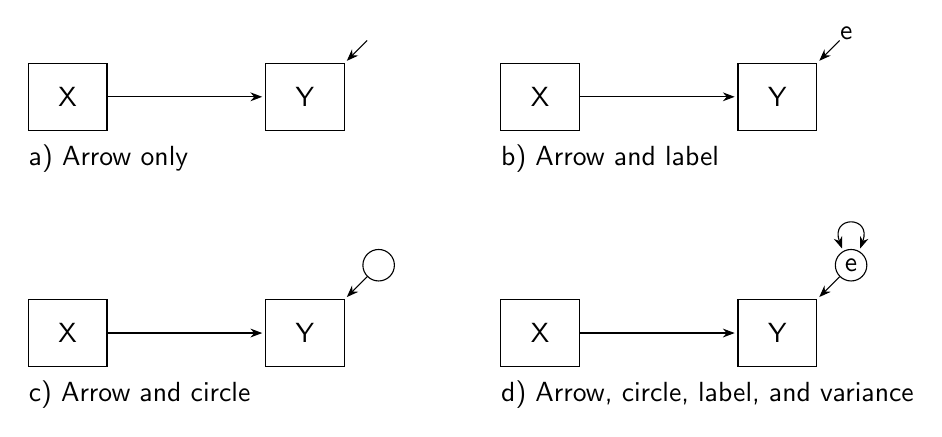
\begin{tikzpicture}

%%% a) Arrow only
\drawmodel{a) Arrow only} 

%% Residual
\node [residual] (e) [above right = 4mm of y] {};
\path [regression] (e) edge (y.north east);


%%% b) Arrow and label
\begin{scope} [xshift = 6cm]
\drawmodel{b) Arrow and label}

%% Residual
\node [residual] (e) [above right = 4mm of y] {e};
\path [regression] (e) edge (y.north east);
\end{scope}


%%% c) Arrow and circle
\begin{scope} [yshift = -3cm]
\drawmodel{c) Arrow and circle}

%% Residual
\node [residual = {0}{4mm}{draw, circle}] (e) [above right = 4mm of y] {};
\path [regression] (e) edge (y.north east);
\end{scope}


%%% d) Arrow, circle, label, and variance
\begin{scope} [xshift = 6cm, yshift = -3cm]
\drawmodel{d) Arrow, circle, label, and variance}

%% Residual
\node [residual = {0}{4mm}{draw, circle}] (e) [above right = 4mm of y] {e};
\path [regression] (e) edge (y.north east);

\path [variance = {right}{110}{6}] (e.60) edge (e.120);
\end{scope}

\end{tikzpicture}
\end{document}
